\section{Validation against NHWAVE following \texorpdfstring{\citet{ma2012}}{Ma et al. (2012)}}
\label{sec:ma2012}
\label{sec:ma}

\subsection{Test programme}
\label{sec:ma-programme}

\citet{ma2012} introduced NHWAVE with seven tests (their Section~4), and the
NHWAVE repository ships examples for several of them.
Table~\ref{tab:ma-programme} lists them with what each one tests and whether
\NHFOAM\ can run it today. Tests 1--4 and 6 need no new physics and were run
with both models on the same set-up; tests 5 and 7 need wetting and drying,
which was added afterwards (Section~\ref{sec:wd}), and test 5 and the
surf-zone example are reported there. The NHWAVE runs use the binary built from the
\code{JimKirby/NHWAVE} master branch (Table~\ref{tab:models}); the reruns of
the paper's own tests check that our NHWAVE runs reproduce the published ones.

\begin{table}[ht]
\centering
\caption{The tests of \citet{ma2012} and their status in \NHFOAM.}
\label{tab:ma-programme}
\small
\begin{tabular}{p{0.6cm}p{4.0cm}p{3.6cm}p{2.5cm}p{2.5cm}}
\toprule
 & test & what it tests & reference & \NHFOAM \\
\midrule
4.1 & standing wave in a closed basin, $kD = \pi$, $2\pi$, $3\pi$ & dispersion with 3--10 layers & linear theory & Section~\ref{sec:ma-basin} \\
4.2 & solitary wave, $H/h = 0.5$, constant depth & nonlinearity, time accuracy & exact solution & Section~\ref{sec:ma-solitary} \\
4.3 & periodic waves over a submerged bar & shoaling, release of harmonics & \citet{luth1994} & Section~\ref{sec:ma-bar} \\
4.4 & elliptic shoal on a 1:50 slope & 3D refraction and diffraction & \citet{berkhoff1982} & Section~\ref{sec:ma-berkhoff} \\
4.5 & breaking solitary wave run-up & breaking, wetting and drying & \citet{synolakis1987} & Section~\ref{sec:wd-runup} \\
4.6 & 3D rigid landslide, $d = 61$ mm & moving bottom, short trailing waves & \citet{enet2007} & Section~\ref{sec:ma-landslide} \\
4.7 & longshore current on a plane beach & breaking-driven currents & \citet{visser1991} & Section~\ref{sec:brk-ls} \\
-- & surf zone (NHWAVE example \code{tingkirby}) & breaking, set-up, undertow & \citet{ting1994} & Sections~\ref{sec:wd-tk}, \ref{sec:brk-spill} \\
\bottomrule
\end{tabular}
\end{table}

The tests were run in order of increasing complexity, and each was used to look
for weaknesses of \NHFOAM\ before moving on. Two of them changed the code and
its defaults: the standing waves showed that the TVD convection scheme damps
steep short waves, and the solitary wave showed that the time integration was
only first order for nonlinear waves (Section~\ref{sec:time}). The surf zone
of \citet{ting1994} later led to the breaking eddy viscosity of
Section~\ref{sec:brk}, which is used for test 4.7. The elliptic
shoal showed when the low-dissipation scheme must not be used, and
Section~\ref{sec:ma-summary} collects all the findings.

\FloatBarrier
\subsection{Standing wave in a closed basin}
\label{sec:ma-basin}

A standing wave of amplitude $a = 0.1$ m and wavelength $L = 20$ m, the length of
the closed basin, is started from rest with $\eta = a\cos kx$. The depth is
$D = 10$, 20 or 30 m, so $kD = \pi$, $2\pi$ or $3\pi$, and $\Delta x = 0.2$ m.
\citet{ma2012} report the normalised rms error at $x = 17.5$ m over 30 s,
\begin{equation}
  \epsilon = \frac{1}{H}\sqrt{\overline{(\eta_a - \eta)^2}},\qquad
  \eta_a = a\cos(kx)\cos(\omega t),\quad H = 2a,
  \label{eq:basinerr}
\end{equation}
for 3, 5, 8 and 10 layers. Both models were run with the same layers; NHWAVE
with its adaptive time step (CFL 0.5), \NHFOAM\ with $\Delta t = 5$ ms.

\begin{table}[ht]
\centering
\caption{Standing wave: normalised rms error \eqref{eq:basinerr} [\%] at
$x = 17.5$ m. LLV: \code{limitedLinearV}; FL2: \code{filteredLinear2V 0.2 0}.}
\label{tab:ma-basin}
\small
\begin{tabular}{llcccc}
\toprule
$kD$ & layers & \citet{ma2012} & NHWAVE, rerun & \NHFOAM, LLV & \NHFOAM, FL2 \\
\midrule
$\pi$ & 3 & 1.63 & 1.69 & 0.65 & 0.56 \\
 & 5 & 0.90 & 0.87 & 0.18 & 0.12 \\
 & 8 & 0.61 & 0.67 & 0.09 & 0.07 \\
 & 10 & 0.53 & 0.60 & 0.11 & 0.11 \\
\addlinespace
$2\pi$ & 3 & 3.07 & 3.05 & 1.08 & 0.16 \\
 & 5 & 1.50 & 1.43 & 0.67 & 0.16 \\
 & 8 & 0.81 & 0.80 & 0.33 & 0.17 \\
 & 10 & 0.64 & 0.66 & 0.24 & 0.17 \\
\addlinespace
$3\pi$ & 3 & 4.90 & 4.81 & 1.28 & 0.25 \\
 & 5 & 2.50 & 2.40 & 1.17 & 0.17 \\
 & 8 & 1.35 & 1.24 & 0.68 & 0.17 \\
 & 10 & 1.00 & 0.94 & 0.48 & 0.17 \\
\bottomrule
\end{tabular}
\end{table}

\begin{figure}[ht]
\centering
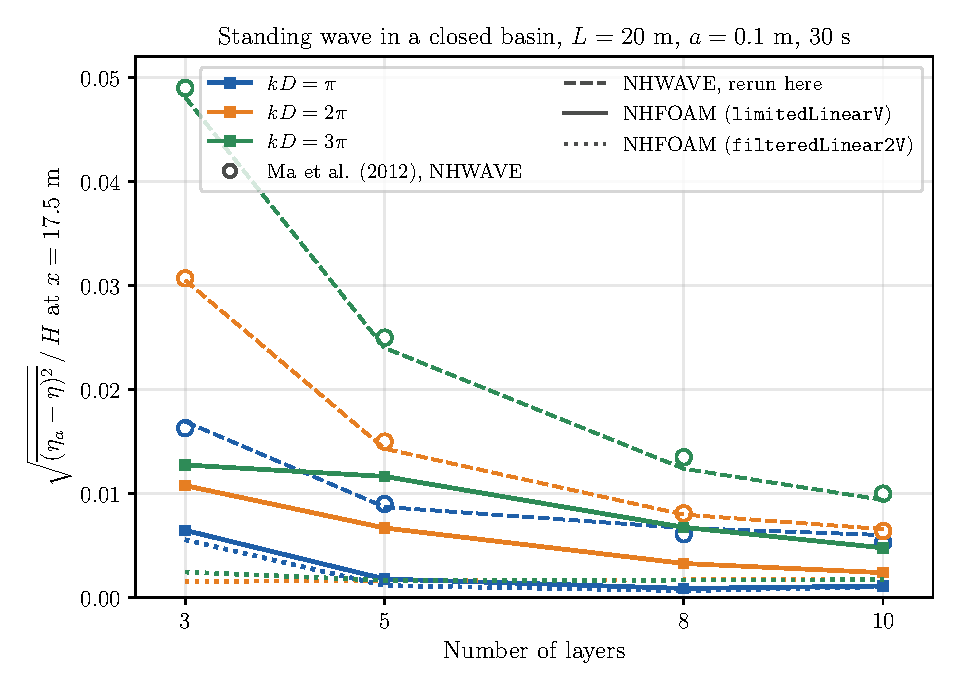
\includegraphics[width=0.8\textwidth]{ma2012_basin.pdf}
\caption{Standing wave in a closed basin: normalised rms error at $x=17.5$ m
against the number of layers. Circles: \citet{ma2012}; dashed: NHWAVE rerun
here; solid and dotted: \NHFOAM\ with the TVD and the filtered central
convection scheme.}
\label{fig:ma-basin}
\end{figure}

Our NHWAVE runs reproduce the published errors to within 0.1 percentage
points (Table~\ref{tab:ma-basin}, Fig.~\ref{fig:ma-basin}), so the NHWAVE
set-up is the paper's. \NHFOAM\ is 2.5--4 times more accurate with the TVD
scheme, and 3--20 times with the filtered central scheme, with which the error
is 0.16--0.25\% for $kD \ge 2\pi$ whatever the number of layers. The remaining
0.56\% at $kD=\pi$ with three layers is the period error of three layers
($-0.07\%$, Section~\ref{sec:dispersion}) accumulated over 8.4 periods.

The difference between the two convection schemes is damping, not phase. The
TVD limiter acts on this wave although its steepness is only $ka = 0.031$: with \code{limitedLinearV} the amplitude at $kD = 3\pi$ with three
layers decays by 8.5\% over 30 s, with \code{filteredLinear2V} by 1.7\%, with
\code{LUST} by 2.8\%. The damping is nonlinear: a wave ten times smaller lost
0.09\%, and halving the time step changed nothing. Repeated with the flux
extrapolation of Section~\ref{sec:time}, the errors of the filtered runs did not
change in the second decimal. This test is the reason
\code{filteredLinear2V} is now recommended for waves that do not break.

\FloatBarrier
\subsection{Solitary wave}
\label{sec:ma-solitary}

A solitary wave of $H/h = 0.5$ travels 150 m over a flat bottom ($h = 1$ m,
$\Delta x = 0.1$ m, 3 layers, 40 s). Its exact shape and velocity field come from
Babenko's equation \citep{babenko1987}, solved with the Petviashvili iteration
\citep{clamond2013} to a residual of $10^{-13}$ (\code{validation/solitary\_exact.py}).
Both models start from the exact $\eta$ and $\bm{u}$; \NHFOAM\ also from the exact
pressure, $\prgh = \tfrac12\left(c^2 - |\bm{u}-c\bm{e}_x|^2\right)$ in the frame
of the wave. NHWAVE runs with CFL 0.5 ($\Delta t \approx 10$ ms), \NHFOAM\ with
$\Delta t = 5$ ms. Table~\ref{tab:ma-solitary} compares the peaks of $\eta$, and of
$u$ and $w$ at mid-depth, with the exact solution after 40 s, and
Fig.~\ref{fig:ma-solitary} shows the profiles.

\begin{table}[ht]
\centering
\caption{Solitary wave, $H/h = 0.5$, 3 layers, $t = 40$ s: error of the peaks of
$\eta$, $u$ and $w$ (mid-depth) and position of the crest relative to the exact
solution. CPU: one core, approximate (runs shared the machine). LLV:
\code{limitedLinearV}; FL2: \code{filteredLinear2V 0.2 0}.}
\label{tab:ma-solitary}
\footnotesize
\begin{tabular}{lccccc}
\toprule
run & $\eta_{\max}$ & $u_{\max}$ & $w_{\max}$ & crest & CPU \\
\midrule
NHWAVE                                            & $-2.3\%$ & $-0.7\%$ & $+0.4\%$ & $-0.08$ m & 570 s \\
\NHFOAM\ before the fix, LLV    & $-6.4\%$ & $-4.3\%$ & $-4.6\%$ & $-0.77$ m & 240 s \\
\quad $2\Delta t$ (10 ms)                         & $-10.3\%$ & $-7.6\%$ & $-9.4\%$ & $-1.37$ m & 110 s \\
\quad $\Delta t/2$ (2.5 ms)                       & $-4.4\%$ & $-2.6\%$ & $-2.2\%$ & $-0.47$ m & 400 s \\
\quad central convection        & $-5.3\%$ & $-3.7\%$ & $-3.5\%$ & $-0.67$ m & 230 s \\
\quad 5 layers                                    & $-5.7\%$ & $-4.2\%$ & $-5.5\%$ & $-0.77$ m & 350 s \\
\quad a non-orthogonal corrector                  & $-6.4\%$ & $-4.4\%$ & $-4.6\%$ & $-0.77$ m & -- \\
\quad 2 outer correctors                          & $-2.3\%$ & $-0.9\%$ & $+0.2\%$ & $-0.17$ m & 390 s \\
\quad 2 outer corr., mesh fixed in the 2nd & $-2.3\%$ & $-0.9\%$ & $+0.2\%$ & $-0.17$ m & 350 s \\
\NHFOAM, flux extrapolation, LLV & $-2.3\%$ & $-0.9\%$ & $+0.3\%$ & $-0.17$ m & 210 s \\
\NHFOAM, flux extrapolation, FL2 & $\bm{-1.0\%}$ & $\bm{-0.2\%}$ & $\bm{+1.6\%}$ & $\bm{-0.07}$ m & 210 s \\
\bottomrule
\end{tabular}
\end{table}

\begin{figure}[ht]
\centering
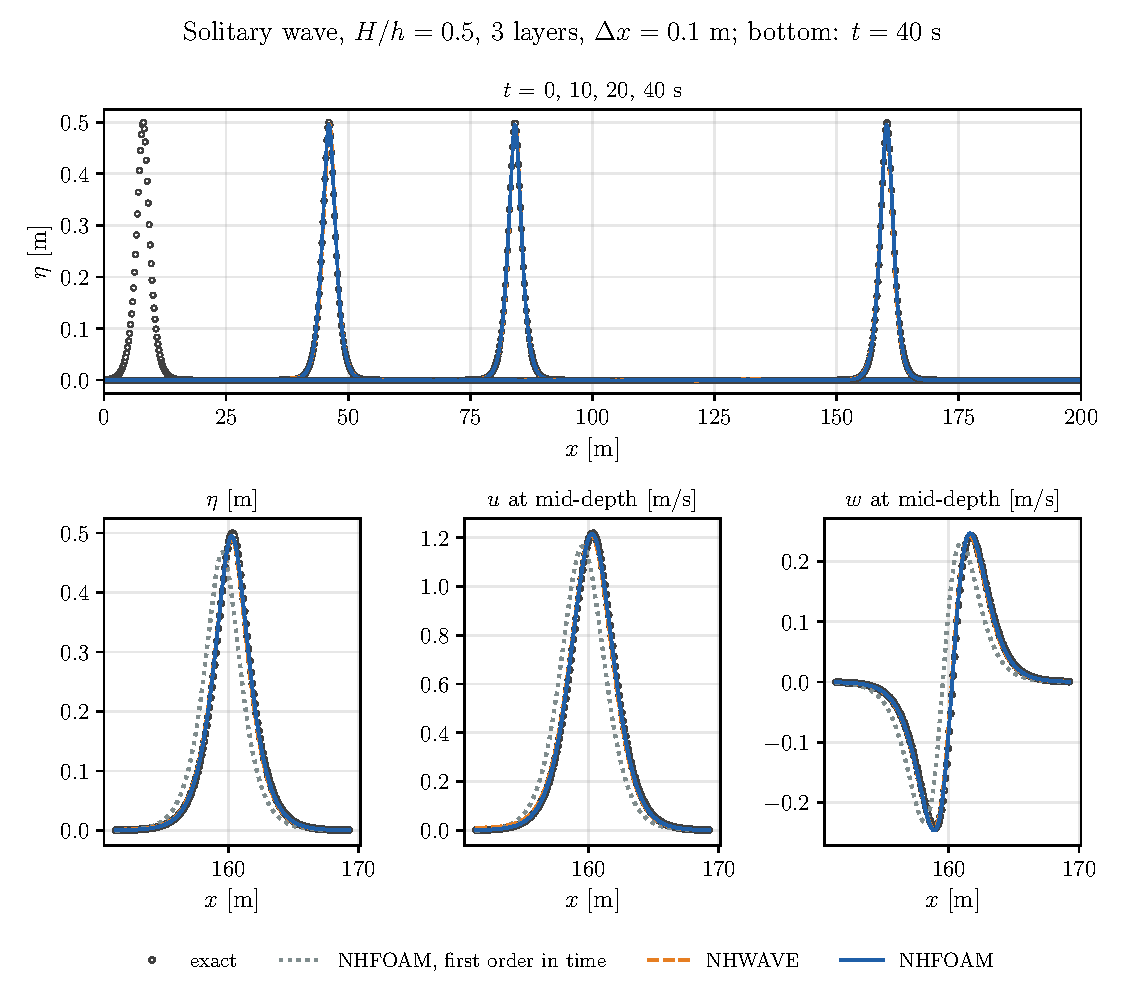
\includegraphics[width=\textwidth]{ma2012_solitary.pdf}
\caption{Solitary wave, $H/h = 0.5$, 3 layers. Top: elevation at $t = 0$, 10, 20
and 40 s. Bottom: $\eta$, $u$ and $w$ at mid-depth around the crest at
$t = 40$ s. \NHFOAM: flux extrapolation and \code{filteredLinear2V}; dotted:
\NHFOAM\ before the fix (one outer corrector, flux of level $n$).}
\label{fig:ma-solitary}
\end{figure}

Before the fix, \NHFOAM\ lost 6.4\% of the wave height in 40 s, three times as
much as NHWAVE, and the crest fell 0.77 m behind. Neither the convection
scheme, the number of layers nor the non-orthogonal correction explained it.
The time step did: the error grew from $-4.4\%$ to $-6.4\%$ and $-10.3\%$ as
$\Delta t$ was doubled twice, i.e.\ linearly in $\Delta t$, and extrapolating
those three runs to $\Delta t\to0$ gives $-2.3\%$ and a lag of 0.17 m. A second
outer corrector gave exactly that, with the mesh moved again in the second
corrector or not. So the cause was not the position of the mesh but the
linearisation of the convection term with the flux of the previous time level
(Section~\ref{sec:time}). Extrapolating the convecting flux \eqref{eq:fluxext}
gives the same result as the second outer corrector at the cost of one, and is
now the default. With it and \code{filteredLinear2V}, the wave keeps its height
after an initial adjustment (about $-1\%$ from $t = 10$ s on) and travels at the
exact speed to within 0.07 m in 150 m. NHWAVE's remaining loss ($-2.3\%$) is the
numerical dissipation of its shock-capturing scheme.

\FloatBarrier
\subsection{Periodic waves over a submerged bar}
\label{sec:ma-bar}

This is NHWAVE's own example (\code{examples/submerged\_bar}), case A of
\citet{luth1994} ($H = 2$ cm, $T = 2.02$ s) with three layers, as in
\citet{ma2012}: a linear boundary wavemaker, a 10 m sponge, $\Delta x = 2$ cm,
CFL 0.5 and, as distributed, a bottom drag coefficient of 0.006. Only the list of
gauges was extended to all ten. \NHFOAM\ runs on the same domain with an 8 m
wave-making zone upstream of NHWAVE's wavemaker, the same sponge, three layers
and $\Delta t = 5$ ms, without bottom friction. Both runs last 40 s and are
compared with the measurements over the last 4 s, with one time shift per run
fitted at $x = 22$ m (Fig.~\ref{fig:ma-bar}, Table~\ref{tab:ma-bar}).

\begin{figure}[p]
\centering
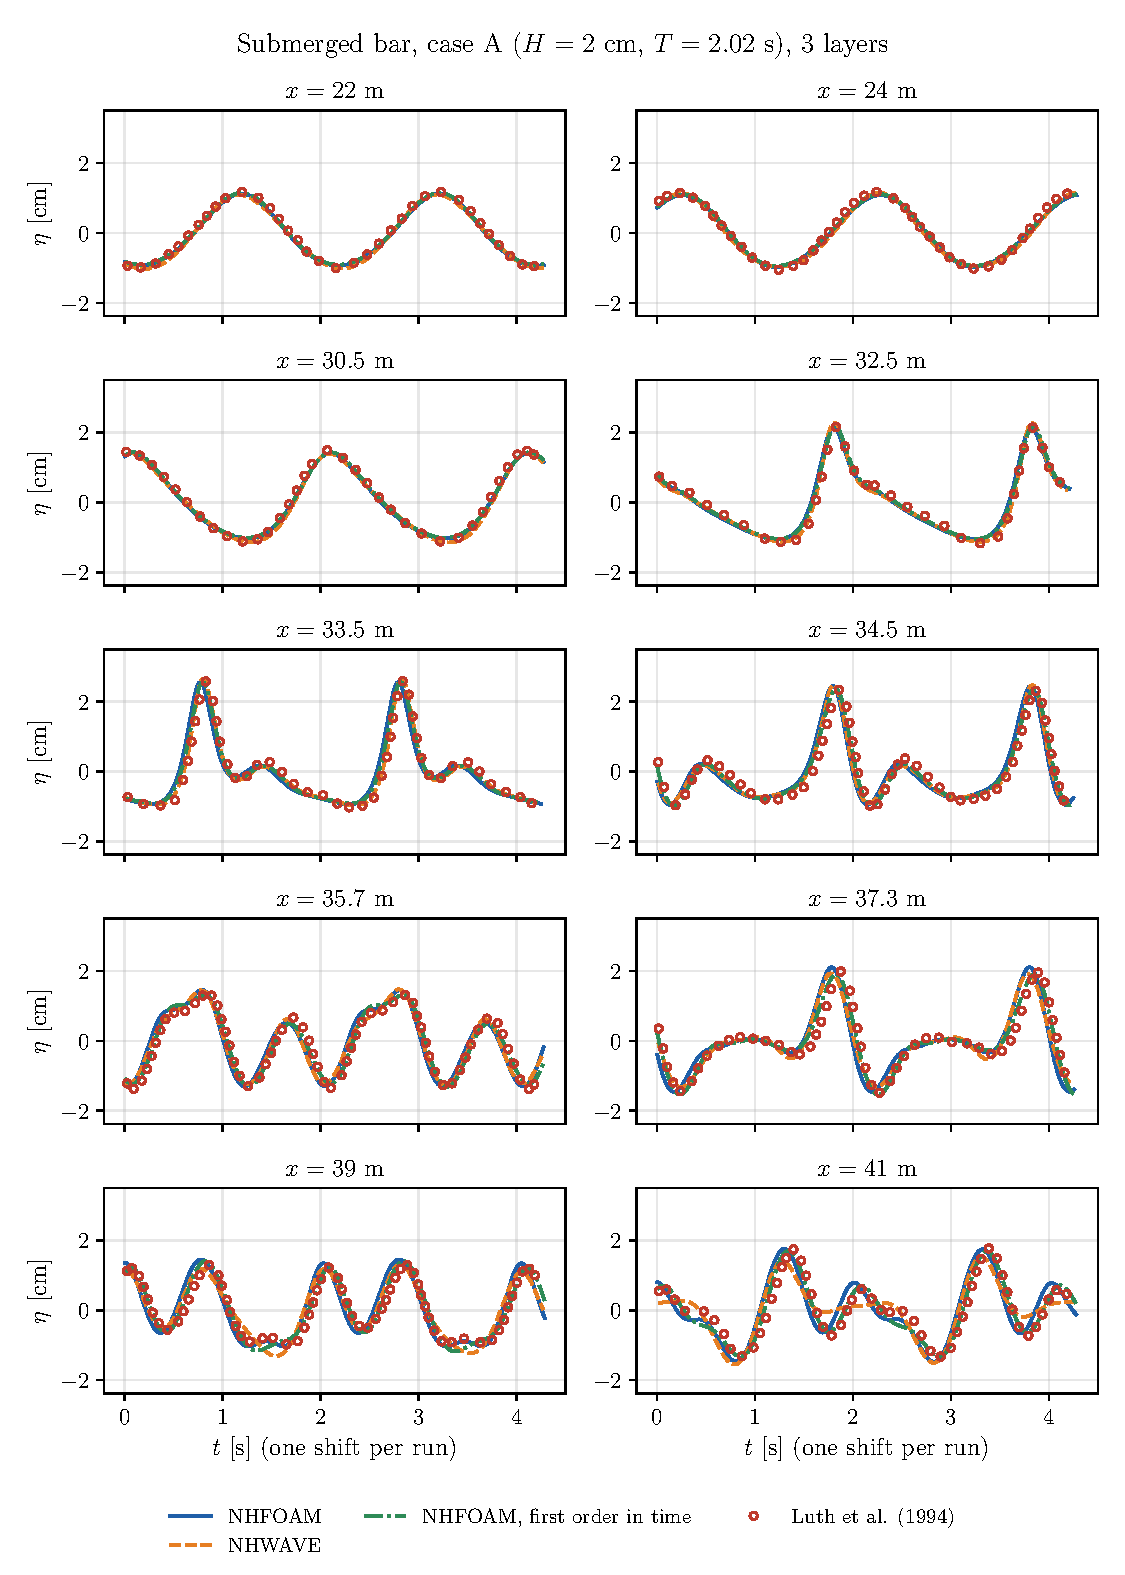
\includegraphics[width=0.9\textwidth]{ma2012_bar.pdf}
\caption{Submerged bar, case A, 3 layers: \NHFOAM\ (flux extrapolation,
\code{filteredLinear2V}), NHWAVE and \NHFOAM\ before the fix of the time
integration, against \citet{luth1994}.}
\label{fig:ma-bar}
\end{figure}

\begin{table}[ht]
\centering
\caption{Submerged bar, case A, 3 layers, window ending at 40 s. Phase: time
shift of the best fit at $x = 35.7$--41 m relative to the shift at $x=22$ m
(negative: the model is early).}
\label{tab:ma-bar}
\small
\begin{tabular}{lccc}
\toprule
 & \NHFOAM & NHWAVE & \NHFOAM\ before the fix \\
\midrule
rms error over the 10 gauges & 0.31 cm & 0.24 cm & 0.16 cm \\
mean $|\Delta H|/H$          & 4.9\%   & 3.8\%   & 4.6\% \\
phase at $x = 35.7$--41 m    & $-0.05$ to $-0.08$ s & $-0.03$ to $-0.08$ s & $-0.01$ to $-0.035$ s \\
\bottomrule
\end{tabular}
\end{table}

Both models reproduce the shoaling on the front slope and the decomposition
into free harmonics behind the bar, with wave heights within a few percent of
the measurements at most gauges. Most of the rms error is phase. After the fix
of the time integration, \NHFOAM's waves over and behind the bar are as early as
NHWAVE's, by up to 0.08 s at the last gauges. Before the fix they were closer to
the measured phase, because the first-order lag slowed them by about 0.5\%, the
same lag that delayed the solitary wave of Section~\ref{sec:ma-solitary}.
With the fix, halving the time step moves the phase by less than 0.005 s, so the
solution is converged in time. The better match of the measured phase before the
fix was therefore a cancellation of errors, and the residual phase error is
shared by both models. Its likely sources are the
linear wave generation, which releases spurious free harmonics, and the long
waves and mean levels of the closed flume (Section~\ref{sec:bar10}). A second
outer corrector, or the TVD instead of the filtered scheme, changes the rms
error by less than 0.02 cm, and the filtered scheme stayed stable over the 40 s
(and over 65 s with ten layers in case C).

\FloatBarrier
\subsection{Elliptic shoal on a sloping bottom}
\label{sec:ma-berkhoff}

The experiment of \citet{berkhoff1982} tests refraction and diffraction in 3D:
an elliptic shoal on a 1:50 slope whose contours are rotated by $20^\circ$
focuses regular waves ($T = 1$ s, $H_0 = 4.64$ cm, $h = 0.45$ m offshore) into a
caustic behind it. The bathymetry is that of \citet{ma2012}, their eqs.\
(49)--(51); it matches the depth file of NHWAVE's example
(\code{examples/berkhoff}) to 2 mm, with the shoal centre at
$(12.025, 10.025)$ m in the coordinates of that example. NHWAVE generates the
waves at its left boundary, absorbs them in a 3 m sponge and has walls at
$y = 0$ and 20 m; \NHFOAM\ has a 3 m wave-making zone upstream of NHWAVE's
wavemaker, the same sponge and walls. To keep the cost of both runs to a few
hours on one core, the grid is twice as coarse as in the paper in both
directions: $\Delta x = 5$ cm and $\Delta y = 10$ cm ($600\times200$ columns),
with three uniform layers (the paper used five). This gives 29 cells per
wavelength offshore and about 18 behind the shoal. NHWAVE runs with CFL 0.5
and, as distributed, a bottom drag coefficient of 0.006; \NHFOAM\ with
$\Delta t = 10$ ms ($T/100$), flux extrapolation and \code{filteredLinear2V}.
Both runs last 30 s, and the wave height is the mean of max $-$ min over the
last five periods at 174 points along the eight measurement sections
(sections 1--5 across the flume at $x = 1$, 3, 5, 7, 9 m behind the shoal
centre, sections 6--8 along it at $y = -2$, 0, 2 m).

Because \NHFOAM\ generates the waves inside a zone and ramps them up over two
periods, its wave train reaches the shoal 2.25 s after NHWAVE's (measured from
the arrival of half the final height at section 1, the same at all its points
to within 0.2 s). Its wave heights are therefore taken over the five periods
ending at $t = 32.25$ s, the same stage of the wave train as NHWAVE's last five
periods ending at 30 s. Figure~\ref{fig:ma-berkhoff} shows the wave heights,
and Table~\ref{tab:ma-berkhoff} the normalised rms error per section,
$\sqrt{\overline{(H_{\mathrm{mod}}-H_{\mathrm{obs}})^2}}\,/\,\overline{H_{\mathrm{obs}}}$,
as defined by \citet{ma2012}.

\begin{figure}[p]
\centering
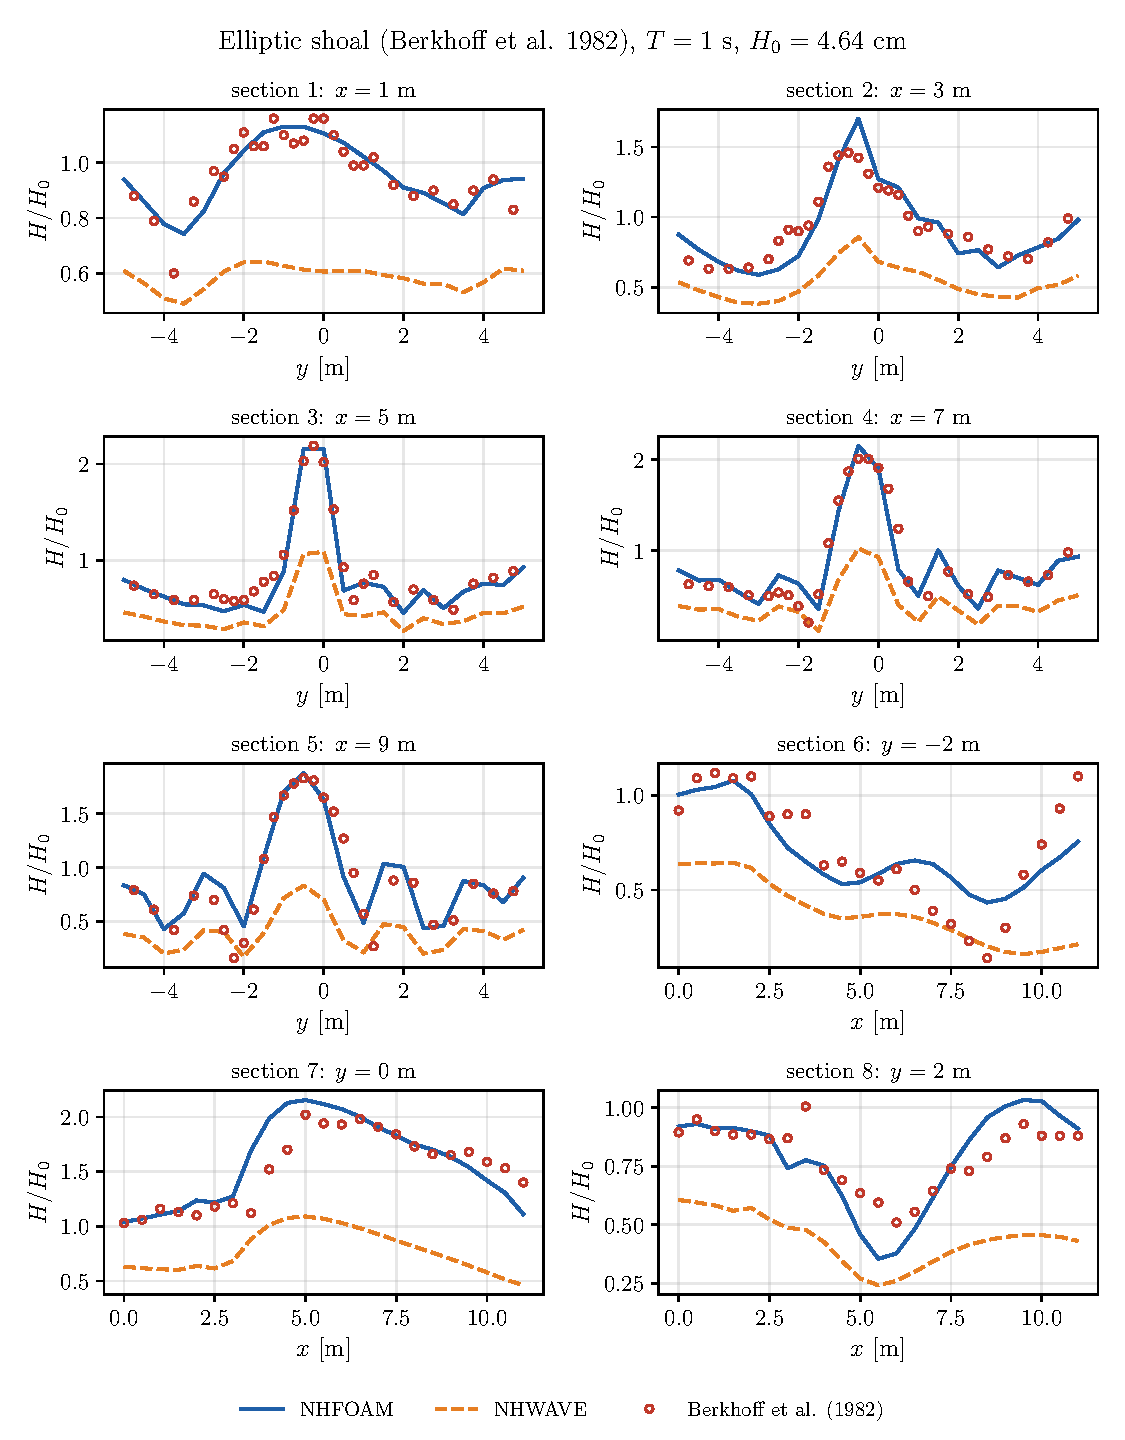
\includegraphics[width=\textwidth]{ma2012_berkhoff.pdf}
\caption{Elliptic shoal: wave height along the eight measurement sections.
\NHFOAM\ and NHWAVE on the same grid ($\Delta x = 5$ cm, $\Delta y = 10$ cm,
3 layers) against \citet{berkhoff1982}.}
\label{fig:ma-berkhoff}
\end{figure}

\begin{table}[ht]
\centering
\caption{Elliptic shoal: normalised rms error of the wave height per
section. \citet{ma2012}: NHWAVE on a grid twice as fine in $x$ and $y$ with five
layers (the paper gives sections 1, 3 and 5 only).}
\label{tab:ma-berkhoff}
\small
\setlength{\tabcolsep}{3.8pt}
\begin{tabular}{lccccccccc}
\toprule
section & 1 & 2 & 3 & 4 & 5 & 6 & 7 & 8 & mean \\
\midrule
\NHFOAM, $\Delta x = 5$ cm         & 0.06 & 0.12 & 0.13 & 0.18 & 0.21 & 0.24 & 0.14 & 0.14 & 0.15 \\
NHWAVE, $\Delta x = 5$ cm          & 0.41 & 0.45 & 0.54 & 0.62 & 0.67 & 0.56 & 0.52 & 0.46 & 0.53 \\
NHWAVE, $\Delta x = 2.5$ cm \citep{ma2012} & 0.07 & -- & 0.11 & -- & 0.11 & -- & -- & -- & -- \\
\bottomrule
\end{tabular}
\end{table}

On this grid \NHFOAM\ reproduces the focusing behind the shoal: the peak of
2.1--2.2 $H_0$ at sections 3 and 4, the side lobes, and the decay along
section 7. At sections 1 and 3 its errors (0.06 and 0.13) are close to those
of NHWAVE on the fine grid of the paper (0.07 and 0.11). NHWAVE on the coarse
grid has the right pattern but only about 60\% of the measured heights: its
incident waves lose 30\% of their height over the first 10 m (from 42.7 mm at
$x = 1$ m to 30.1 mm at $x = 11$ m at $t = 30$ s, along $y = 5$ m), while
\NHFOAM's lose 5\% (46.5 to 44.1 mm, partly by refraction). At 29 cells per
wavelength the shock-capturing scheme of NHWAVE is too dissipative, and it
needs the paper's grid. \NHFOAM\ comes close to the paper's accuracy at
sections 1 and 3 with a quarter of the columns; at section 5 its error is twice
the paper's (0.21 against 0.11). The errors at sections 1--3 change by less than
0.02 when the window is moved by $\pm1$ s, those at sections 4--8, farther from
the wave-maker, by up to 0.08: there the wave train is not yet fully established
by $t\approx 32$ s (in NHWAVE, by 30 s), and a longer run would be needed.

The \NHFOAM\ run itself failed at $t\approx35$ s, after the analysis window
and outside the measurement area. In the shallow corner of the domain at the
south wall, where the depth reaches its minimum of 0.07 m from $x\approx22.7$ m
on, the shoaled waves reach $H/h \approx 1$ and break, and the filtered central
scheme without a breaking model cannot carry the resulting bores
(Section~\ref{sec:convection}). Restarted from $t = 30$ s with
\code{limitedLinearV} and the hydrostatic front approximation, the run went on
to 37 s with up to 171 breaking columns in that corner. The mean error over the
sections at the window ending at 34.5 s was the same for both runs (0.17), and
it fell to 0.14 by 37 s as the wave train at the far sections became
established. A domain in which waves break anywhere, even outside the region of
interest, therefore needs the TVD scheme and the breaking model.

\FloatBarrier
\subsection{3D rigid landslide}
\label{sec:ma-landslide}

\citet{ma2012} used the $d = 61$ mm case of \citet{enet2007}, which was already
compared in Section~\ref{sec:seabed}. It was rerun with the fixed time
integration and \code{filteredLinear2V}, on the same mesh (5 layers,
$\Delta x = \Delta y = 2.5$ cm, the domain ending in a wall 0.2 m from the
shoreline) and against the same NHWAVE run (3 layers, $\Delta x = 2$ cm, full
beach). Figure~\ref{fig:ma-landslide} and Table~\ref{tab:ma-landslide} show the
result.

\begin{figure}[ht]
\centering
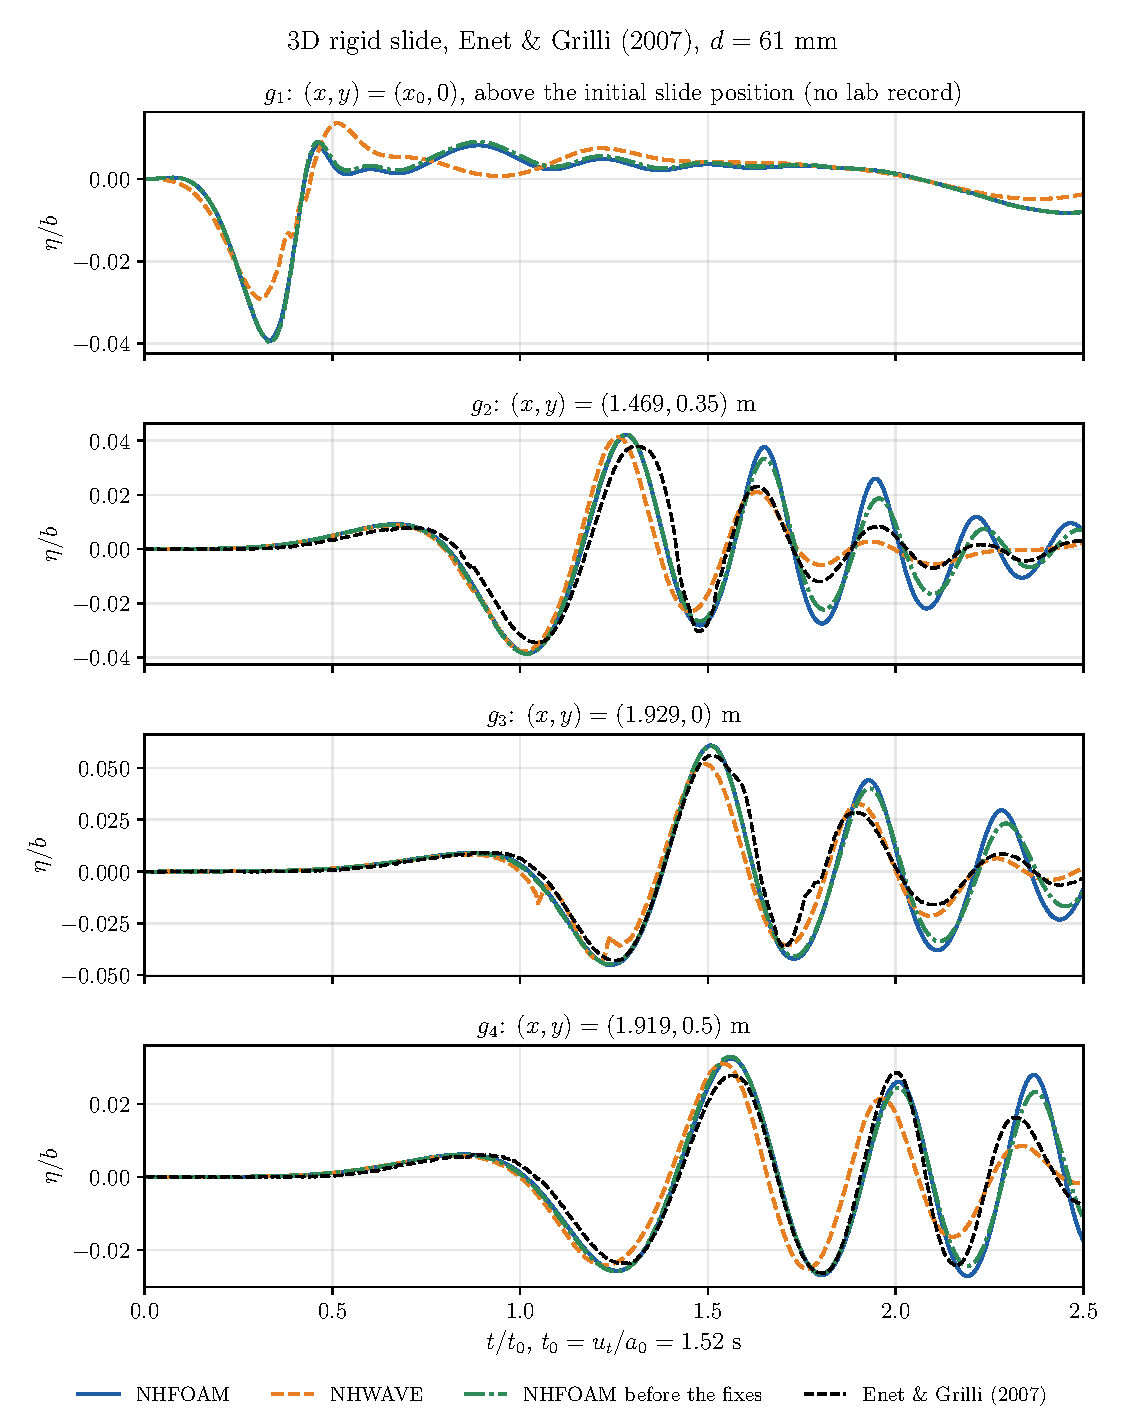
\includegraphics[width=0.85\textwidth]{ma2012_landslide.pdf}
\caption{3D rigid landslide, $d = 61$ mm: \NHFOAM\ with the fixes, NHWAVE and
\NHFOAM\ before the fixes, against \citet{enet2007}.}
\label{fig:ma-landslide}
\end{figure}

\begin{table}[ht]
\centering
\caption{3D rigid landslide, $d = 61$ mm: the largest crest and the two crests
after it [mm] (maxima between zero up-crossings, $t < 2.5\,t_0$).}
\label{tab:ma-landslide}
\small
\begin{tabular}{lccc}
\toprule
 & g2 (1.469, 0.35) & g3 (1.929, 0) & g4 (1.919, 0.5) \\
\midrule
lab                       & 15.0, 9.1, 3.3  & 22.2, 11.3, 3.5 & 11.3, 6.4, -- \\
\NHFOAM                   & 16.7, 14.9, 10.3 & 24.1, 17.4, 11.7 & 12.8, 10.3, 11.1 \\
\NHFOAM\ before the fixes & 16.7, 13.2, 7.4  & 23.9, 15.9, 9.2  & 13.0, 9.7, 9.2 \\
NHWAVE                    & 16.3, 8.3, 1.1   & 20.5, 12.9, 2.5  & 12.3, 8.5, 3.4 \\
\bottomrule
\end{tabular}
\end{table}

The leading trough and crest change by less than 2\%: they are long waves,
and the time integration and the convection scheme hardly affect them. The
trailing waves were too large before the fixes, and they are 10--25\% larger
now that the numerical damping is smaller: the second crest is 1.5 times the
measured one and the third about three times, while NHWAVE follows the measured
decay. The excess is therefore not numerical damping that \NHFOAM\ lacks; its
likely cause is the wall that replaces the beach 0.2 m from the shoreline. The
slide also sends waves towards the shore. In \NHFOAM\ they are reflected by
the wall, less than 0.4 m shoreward of the slide, and come back to the gauges at
about $t \approx 1.5\,t_0$, when the excess starts; on NHWAVE's beach they run
up and are partly dissipated. This test
needs the beach to be conclusive; with the wetting and drying of
Section~\ref{sec:wd} it can now be rerun with it.

\paragraph{With the beach.} The run was repeated with the slope continued
0.25 m inland of the still-water shoreline (the bed 6.7 cm above the still
water) and wetting and drying (5 mm film), otherwise unchanged (147\,600
cells; Fig.~\ref{fig:ma-landslide-beach}). The leading trough and crest
change by less than 4\%, and the trailing waves are no smaller: the
largest crest and the two after it are 17.3, 15.7 and 10.7 mm at g2
(wall: 16.7, 14.9, 10.3), 23.4, 18.2 and 11.3 mm at g3 (24.1, 17.4, 11.7)
and 12.7, 11.6 and 10.7 mm at g4 (12.8, 10.3, 11.1). The wall is therefore
not the cause of the excess. The trailing waves ($kh = 3$--5) follow the
convection scheme instead: they were smaller with the more dissipative TVD
scheme before the fixes, and NHWAVE's shock-capturing scheme damps them
most. Whether the measured decay of the trailing waves is physical damping
that an inviscid model lacks, or comes from details of the slide motion,
remains open.

\begin{figure}[!htbp]
\centering
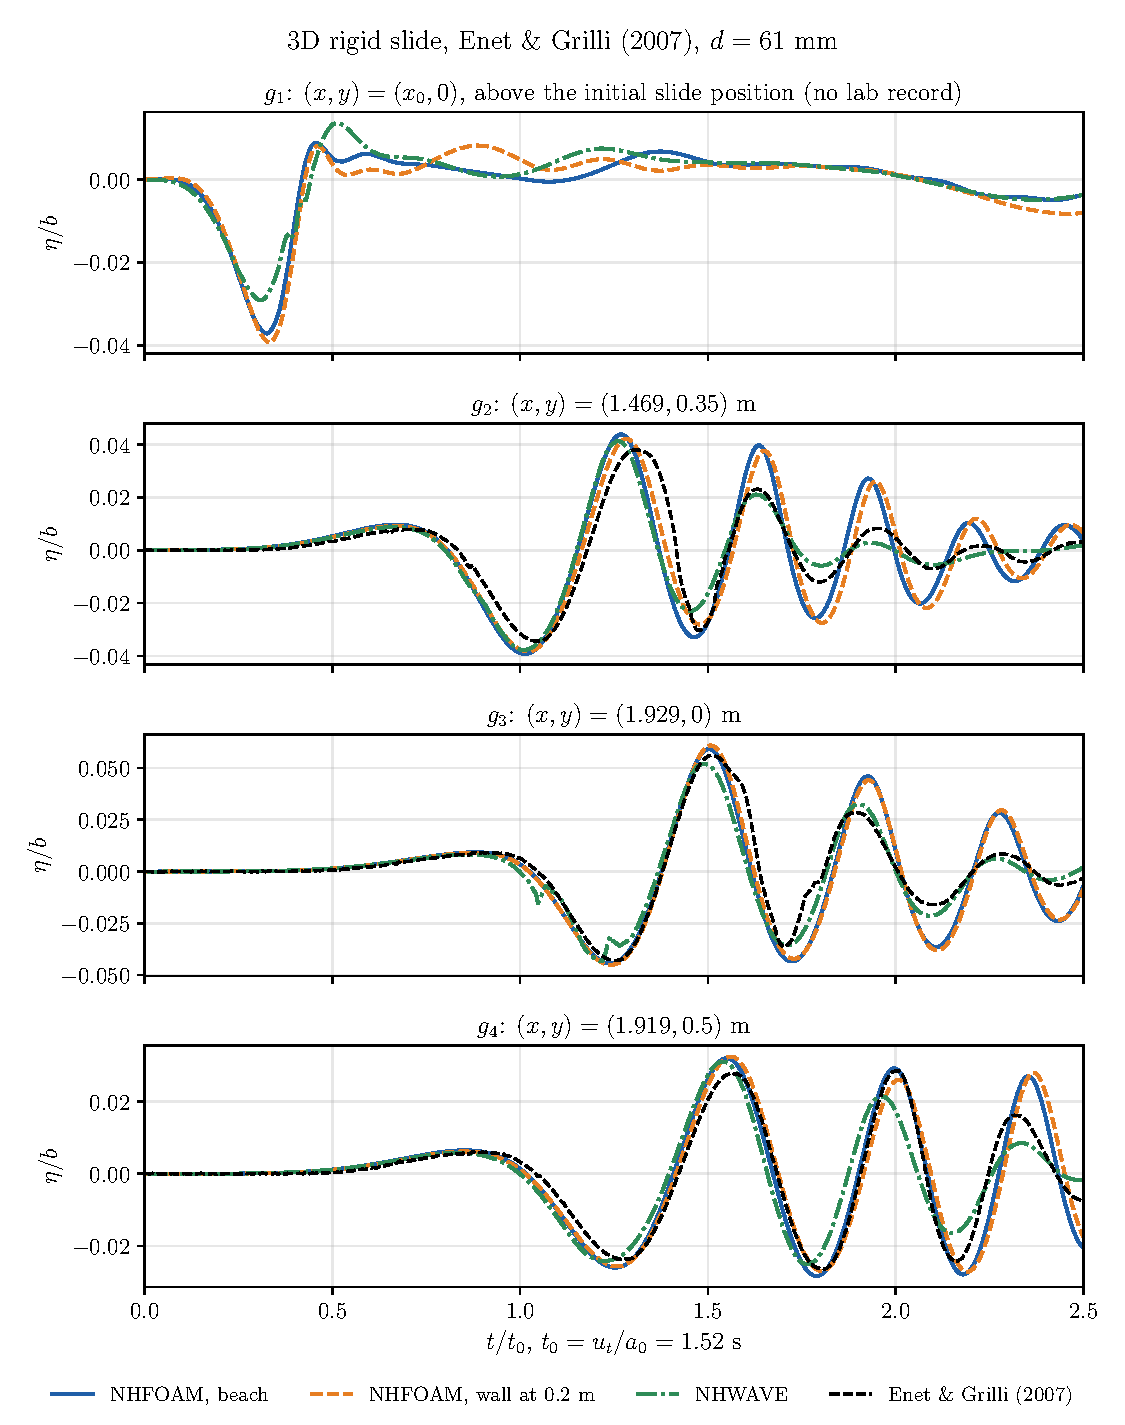
\includegraphics[width=0.85\textwidth]{landslide_beach.pdf}
\caption{3D rigid landslide, $d = 61$ mm: \NHFOAM\ with the beach and
wetting and drying, with the wall 0.2 m from the shoreline, and NHWAVE,
against \citet{enet2007}.}
\label{fig:ma-landslide-beach}
\end{figure}

\FloatBarrier
\subsection{Summary of the problems found and their fixes}
\label{sec:ma-summary}

Table~\ref{tab:fixes} lists the weaknesses that the comparisons with NHWAVE
exposed, here and in Section~\ref{sec:verification}, with their causes and
fixes.

\begin{table}[ht]
\centering
\caption{Problems found by the tests and their fixes.}
\label{tab:fixes}
\small
\begin{tabular}{p{2.3cm}p{3.6cm}p{3.6cm}p{4.6cm}}
\toprule
test & problem & cause & fix and effect \\
\midrule
dispersion (Section~\ref{sec:dispersion}) & 10--20 layers needed for $kh = 4$--7 & cell-centred pressure & pressure on the layer interfaces: 2 layers for $kh \le 7$ \\
3D landslide (Section~\ref{sec:seabed}) & DIC breaks down with thick layers & matrix not diagonally dominant & \code{sigmaColumn} line preconditioner \\
breaking (Section~\ref{sec:breaking}) & pressure correctors diverge under bores & lagged vertical pressure difference through sloping mid-planes & over-relaxed split \eqref{eq:midflux} \\
standing wave (Section~\ref{sec:ma-basin}) & short steep waves damped (8.5\% in 30 s) & TVD limiter & \code{filteredLinear2V} for non-breaking waves: error 0.16--0.25\% for $kD\ge2\pi$ \\
solitary wave (Section~\ref{sec:ma-solitary}) & height $-6.4\%$, crest 0.77 m late in 150 m & convecting flux of level $n$: first order in time & flux extrapolation \eqref{eq:fluxext}: $-1.0\%$, 0.07 m, no extra cost \\
submerged bar (Section~\ref{sec:ma-bar}) & phase closer to the lab before the fix & the first-order lag cancelled an error shared with NHWAVE & none yet; the phase now agrees with NHWAVE \\
submerged bar, long runs (Section~\ref{sec:bar-bc}) & phase drifts by 0.21 s in 20 s & no return current in the wave-making zone & return current (default), or the boundary wavemaker: no drift, steady 1.0 cm error \\
elliptic shoal (Section~\ref{sec:ma-berkhoff}) & run fails at 35 s in a shallow corner & waves break there; filtered scheme, no breaking model & \code{limitedLinearV} and HFA wherever waves break: the run goes on, same errors \\
landslide (Section~\ref{sec:ma-landslide}) & trailing waves 1.5--3 times too large & not the wall: the run with the beach gives the same & open \\
run-up (Section~\ref{sec:wd-runup}) & front too slow, $R/d = 0.41$; oscillating swash & centred face depth, interpolated flux at the tip & upwind (TVD) face depth, supercritical upwind flux: $R/d = 0.531$ (NHWAVE 0.512) \\
surf zone (Section~\ref{sec:wd-tk}) & heights 6 cm too large at $x = 8$ m & too little dissipation behind the hydrostatic front & breaking age and eddy viscosity (Section~\ref{sec:brk}): mean surf-zone error $+6.1 \to +3.5$ cm (NHWAVE $+4.8$) \\
longshore current (Section~\ref{sec:brk-ls}) & breaking region crept into deep water along oblique crests & columns joined at the aged threshold & join at $\beta\sqrt{gD}$ \\
\bottomrule
\end{tabular}
\end{table}
